\pagebreak
\printbibliography


\pagebreak
\section{Appendix}
\appendix


\section{Deployment View}
See next page
\label{appendix:DeploymentView}
\incgraph[documentpaper]
  [width=\paperwidth,height=\paperheight]{images/DeploymentView2.0.jpg}

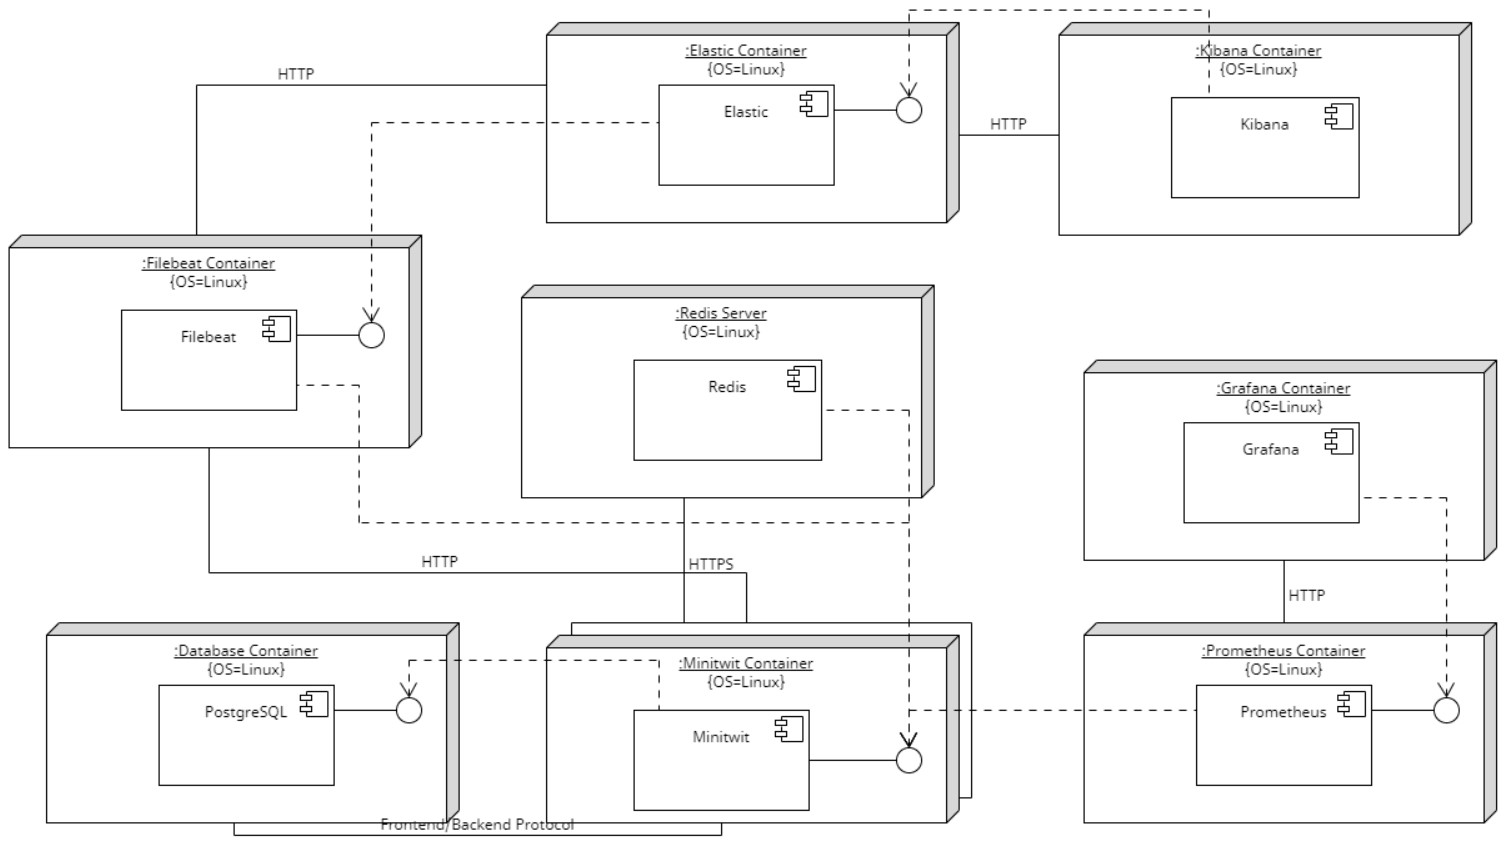
\includegraphics[width=1\textwidth]{images/DeploymentView2.0.jpg}
\section{Hand over guide}
\label{appendix:handOverGuide}
Parts that need to be set up to inherit the codebase and deploy to a cloud server:
\begin{itemize}
    \item Local envionment variables: SSH\_KEY\_NAME, DIGITAL\_OCEAN\_TOKEN and AUTH\_KEY\_HEARTBEAT.
    \item GitHub Action Secrets: SSH\_HOST and STAGING\_SSH\_HOST.
\end{itemize}
To then deploy to a cloud server (in DigitalOcean), the "cloud\_deployment.md" guide in the GitHub repository should be followed.

In case the whole project is taken over, the following GitHub Actions Secrets would need to be set up:
\begin{itemize}
    \item DOCKER\_PASSWORD
    \item DOCKER\_USERNAME
    \item ELASTICSEARCH\_PASSWORD
    \item ENCRYPTION\_KEY
    \item PAT
    \item POSTGRES\_DB
    \item POSTGRES\_PASSWORD
    \item POSTGRES\_PORT
    \item POSTGRES\_SERVER
    \item POSTGRES\_USER
    \item POSTMAN\_API\_KEY
    \item REDIS\_HOST
    \item REDIS\_PASSWORD
    \item REDIS\_PORT
    \item SESSION\_SECRET\_KEY
    \item SSH\_HOST
    \item SSH\_KEY
    \item SSH\_USER
    \item STAGING\_SSH\_HOST
\end{itemize}

\section{Security Assessment (Partner Group)}
\label{appendix:securityAssessment}

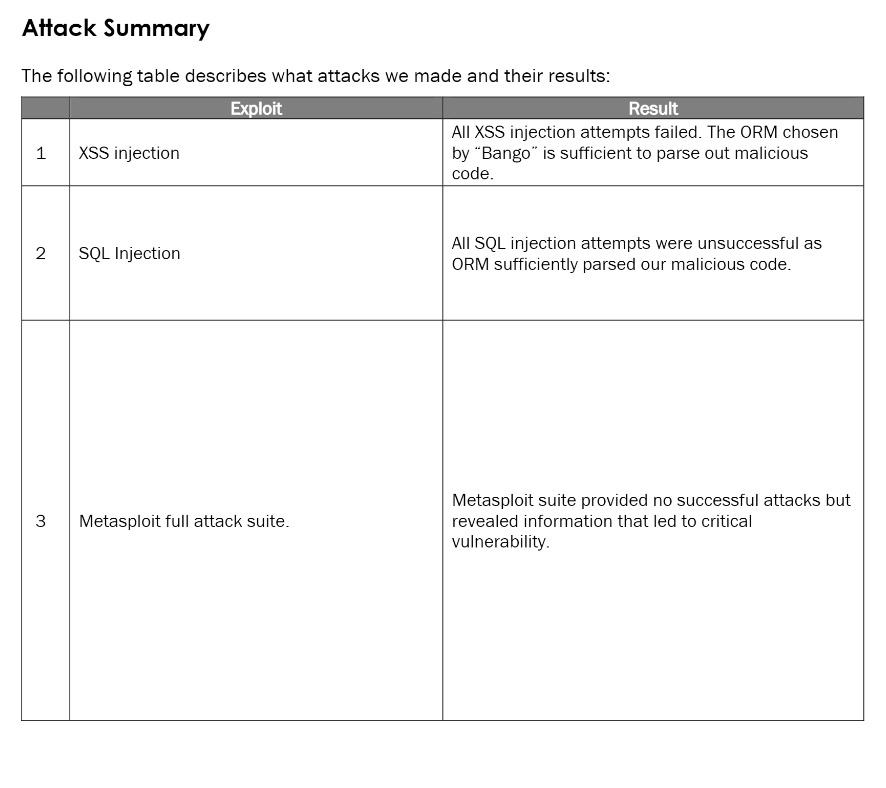
\includegraphics[width=1\textwidth]{images/Attack P1.png}

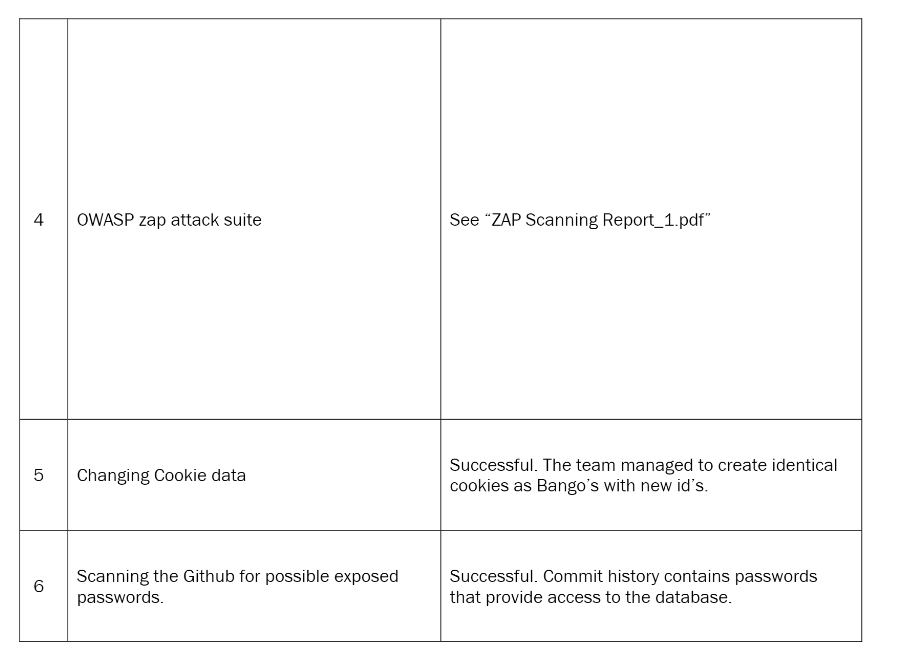
\includegraphics[width=1\textwidth]{images/Attack P2.png}


\section{Monitoring Dashboard}
\label{appendix:monitoringDashboard}
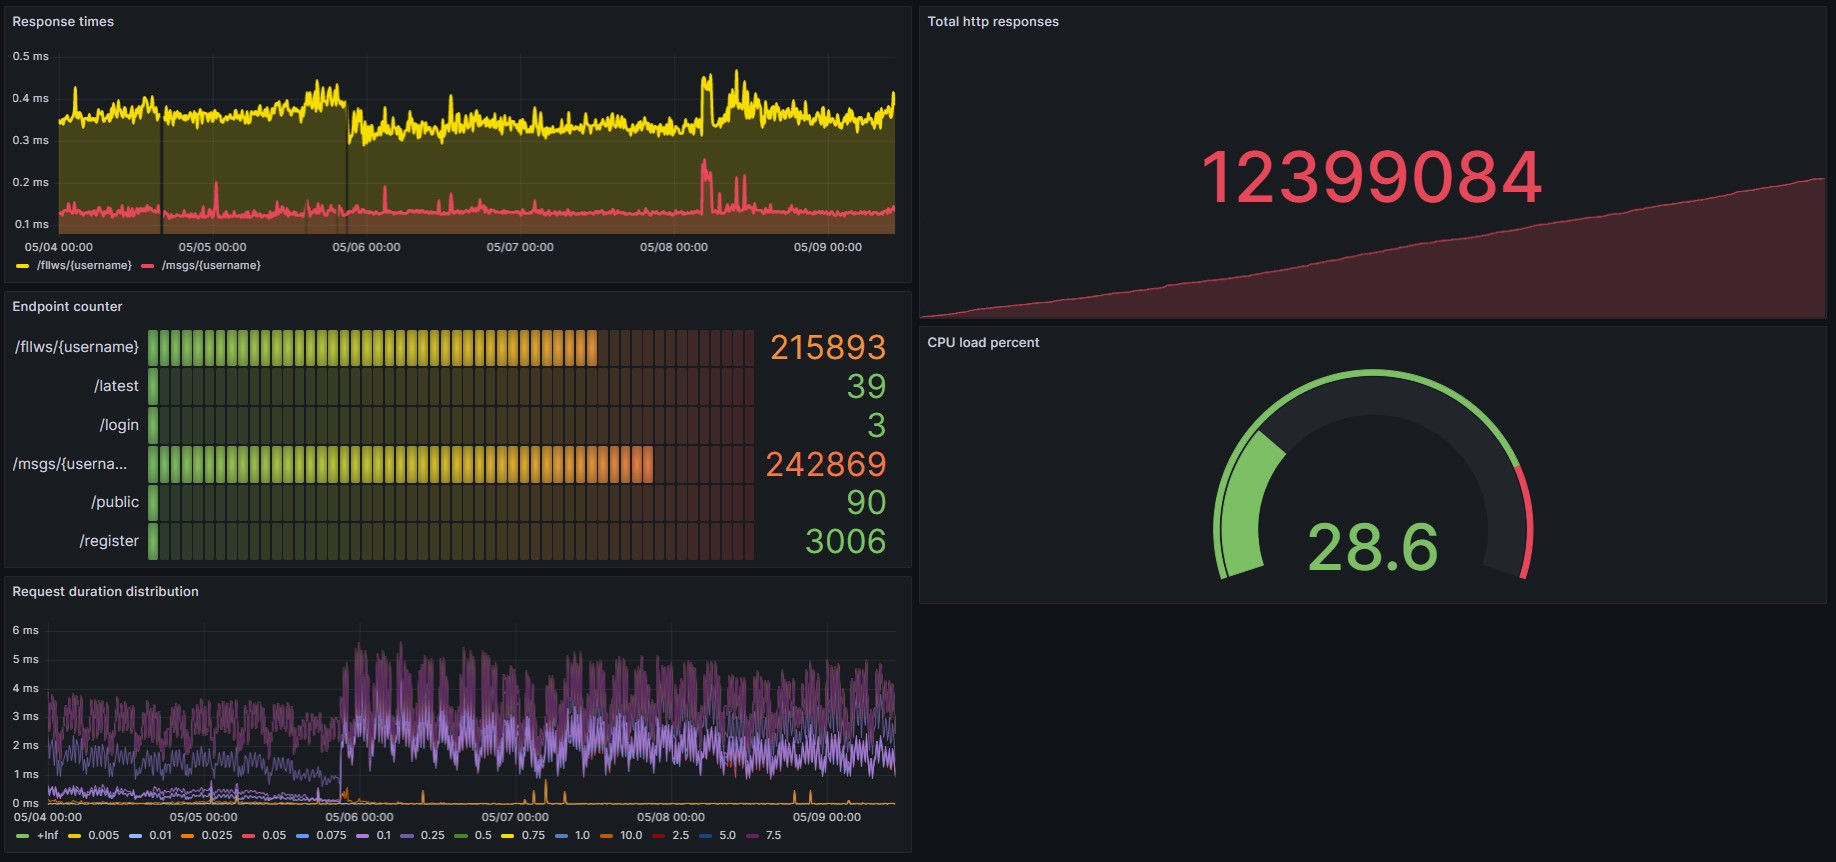
\includegraphics[width=1\textwidth]{images/MonitoringDashboard.jpg}

\section{Logging Dashboard}
\label{appendix:loggingDashboard}
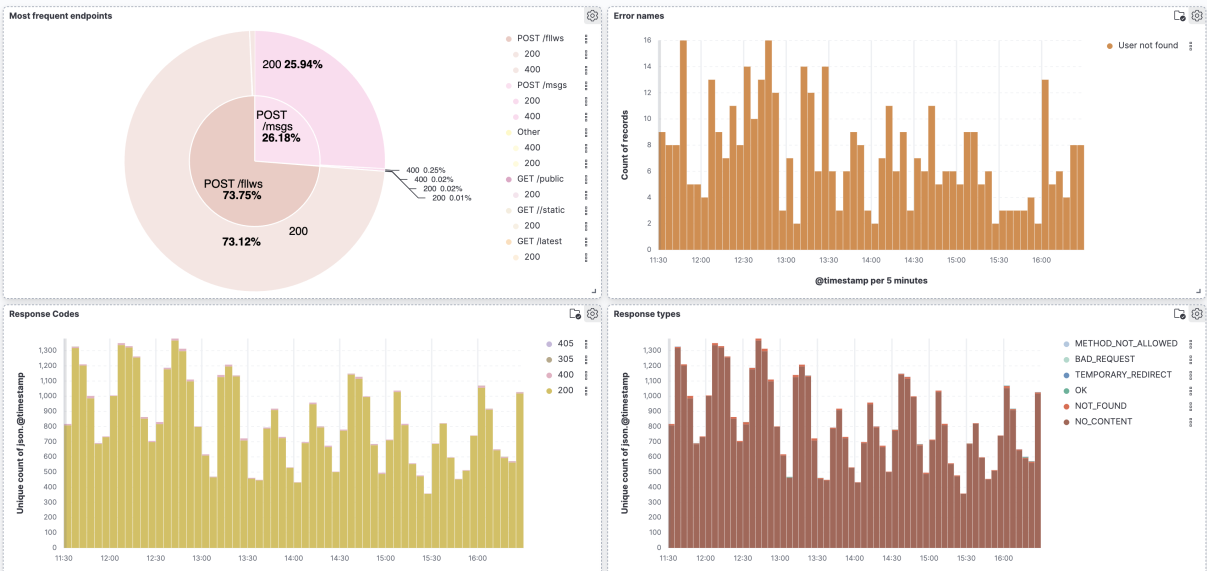
\includegraphics[width=1\textwidth]{images/LoggingDashboard.png}
